\documentclass[tikz,border=2pt]{standalone}
\usepackage{amsmath,amssymb}
\usepackage{pgfplots}
\pgfplotsset{compat=1.18}

\begin{document}
% Memoryless: having survived to time s, the remaining lifetime has the same distribution as
% a fresh one. The tail of the exponential survival curve beyond s, rescaled to start at 1,
% is the original curve again.
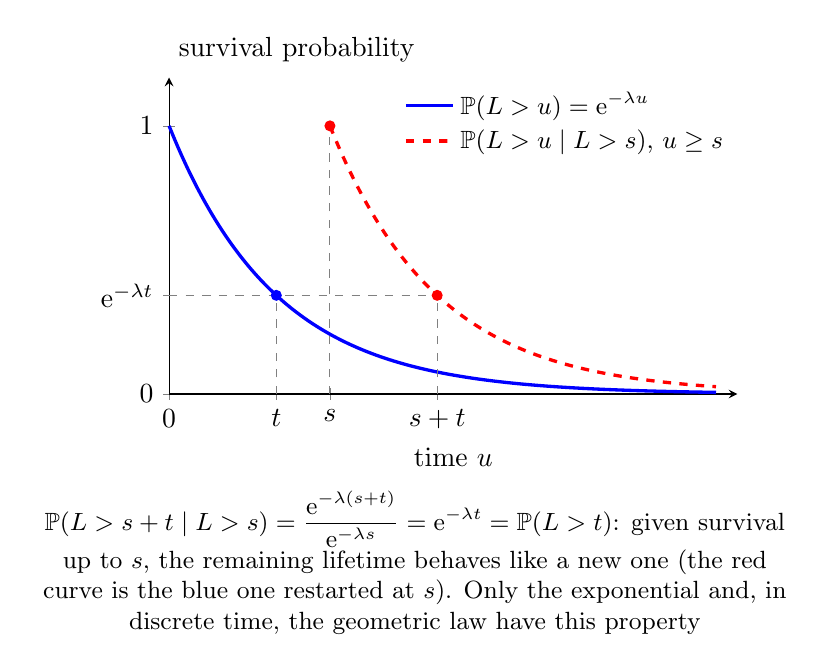
\begin{tikzpicture}
	\begin{axis}[
		axis lines=left, xmin=0, xmax=5.3, ymin=0, ymax=1.18,
		xtick={0,1,1.5,2.5}, xticklabels={$0$,$t$,$s$,$s+t$}, ytick={0,0.368,1}, yticklabels={$0$,$\mathrm{e}^{-\lambda t}$,$1$},
		xlabel={time $u$}, ylabel={survival probability}, ylabel style={rotate=-90, anchor=south west, at={(axis description cs:0,1.02)}},
		samples=120, smooth, width=8.8cm, height=5.6cm, clip=false,
		legend style={draw=none, fill=none, font=\small, at={(1.0,0.99)}, anchor=north east}, legend cell align=left
		]
		\addplot[blue, very thick, domain=0:5.1] {exp(-x)};
		\addlegendentry{$\mathbb{P}(L>u)=\mathrm{e}^{-\lambda u}$}
		\addplot[red, very thick, dashed, domain=1.5:5.1] {exp(-(x-1.5))};
		\addlegendentry{$\mathbb{P}(L>u\mid L>s)$, $u\ge s$}
		\draw[gray, dashed] (axis cs:1.5,0) -- (axis cs:1.5,1.0);
		\draw[gray, dashed] (axis cs:2.5,0) -- (axis cs:2.5,0.368);
		\draw[gray, dashed] (axis cs:1,0) -- (axis cs:1,0.368);
		\draw[gray, dashed] (axis cs:0,0.368) -- (axis cs:2.5,0.368);
		\fill[blue] (axis cs:1,0.368) circle (2pt);
		\fill[red] (axis cs:2.5,0.368) circle (2pt);
		\fill[red] (axis cs:1.5,1) circle (2pt);
	\end{axis}
	\node[anchor=north, font=\small, align=flush center, text width=9.6cm] at ([yshift=-2pt]current axis.outer south) {$\mathbb{P}(L>s+t\mid L>s)=\dfrac{\mathrm{e}^{-\lambda(s+t)}}{\mathrm{e}^{-\lambda s}}=\mathrm{e}^{-\lambda t}=\mathbb{P}(L>t)$: given survival up to $s$, the remaining lifetime behaves like a new one (the red curve is the blue one restarted at $s$). Only the exponential and, in discrete time, the geometric law have this property};
\end{tikzpicture}
\end{document}
